%************************************************
\chapter{Conclusion and future outlook}\label{ch:outlook} % $\mathbb{ZNR}$
%************************************************
In the present work, we introduced and implemented an alternative paradigm for the flash generation of events at the CMS experiment, based on state-of-the-art results from the ML field.

We were able to successfully simulate physical target distributions with great accuracy, preserving the correct correlations between them and demonstrating that our method is capable of varying the output results according to the physical information provided as input. This conditioning has been compared to that of the other competing approach for fast simulation, CMS FastSim, and has been shown to provide more accurate and precise results when compared with the original FullSim target for b-tag discrimination and jet $p_T$ resolution. Additionally, the proposed solution has demonstrated decisive advantages in terms of speed, with orders of magnitude of speed-up.

We also built a first prototype for an end-to-end sample generator in the standard CMS NanoAOD format, and actually deployed it at scale on millions of events, coming from the training process as well as new, previously unseen ones. 

Finally, we demonstrated that the results obtained can be used in a real world scenario such as a complex, multivariate, MC based analysis as the VBF Channel of H$\rightarrow\mu^+\mu^-$. We computed the key derived quantities for the analysis for both the FullSim and the FlashSim samples, and we observed comparable results on the evalutation of the DNN classifier used in the corresponding CMS publication.
Our approach was also able to provide interesting results regarding the generation of samples to be used as systematic variations when a FullSim reference exists, correctly reproducing the differences between competing approaches such as \texttt{POWHEG} and \texttt{MadGraph5\_aMC@NLO}. The speed of the proposed approach allowed us to make use of all the Gen-level information as well, through the technique of upsampling.

\section{Towards a complete FlashSim}
This work has also emphasized some limitations and peculiarities of the selected approach, pointing to the next steps to be taken if the CMS Collaboration were to adopt the proposed method.

The two major ones are discussed below.


\subsection{Building a full NanoAOD}
A full scale FlashSim must be able of reproducing the content of a NanoAOD file in its entirety. Due to the hundreds of variables stored in a single Event, the most reasonable approach is the one taken in the present work: instead of devising a massive single model for generating all the variables, it is better to divide the problem into a collection of separate physical objects, each reconstructed through its own network.

This has the clear advantage of reducing the size of the models and the resources needed for their trainings, beside, each single model may be conditioned on relevant quantities coming either from the Gen-level, from other model outputs or being specifically engineered to communicate key information regarding the event.

One crucial element for the production of convincing NanoAODs is the presence of \emph{fakes}. The stochastic nature of these objects make their production non-trivial, however there exist other techniques from the ML field, such as \emph{LSTM} \cite{lstm}, for handling and generation of variable-length sequences. The generation would depend on key quantities such as the PileUp and the GenParticles.

Another key quantity, the \emph{Missing Transverse Energy} (MET), could also depend on the final-state reconstructed objects, as this would allow us to obtain a more consistent description of the whole event.

A possible global picture, with multiple dependencies and conditionings, is illustrated in Figure \ref{fig:globpic}.

\begin{figure}
    \centering
    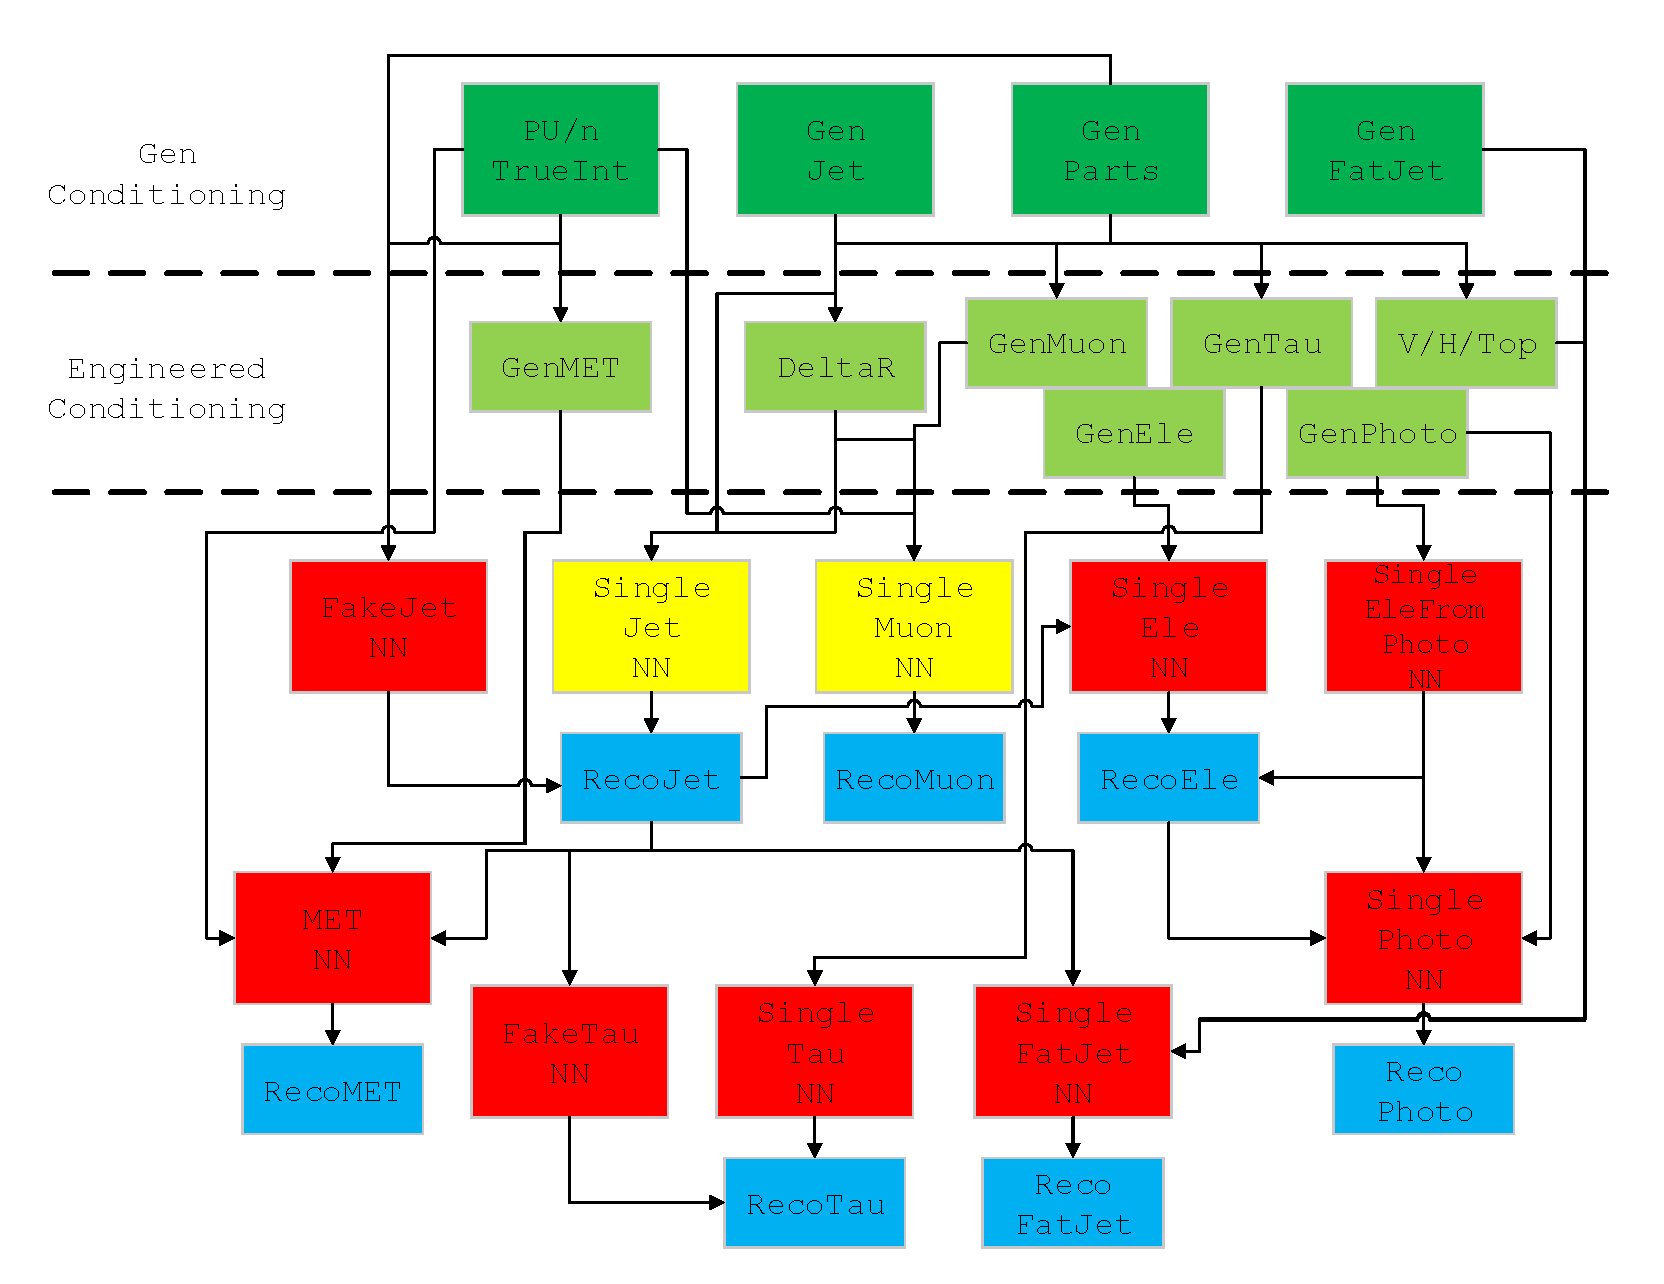
\includegraphics[width=\linewidth]{gfx/ch7/fullnanoaod.pdf}
    \caption[A global picture]{A possible global picture illustrating the various dependencies between conditioning, single object networks and RECO outputs.}
    \label{fig:globpic}
\end{figure}

\subsection{Optimization}
An important series of steps in the prototype end-to-end generator need to be optimized. 
First of all, the Gen-level quantities currently extracted from existing FullSim NanoAODs and written to file for processing could be produced from a dedicated FlashNano-Generator, capable of passing the desired inputs directly to our models without the need of previously existing files.

The ML models forming the backbone of our approach need to be properly optimized and thoroughly examined to find the best combination of hyperparameters, size and performance. Additionally, the training and the generation procedure may be modified to be run in parallel over multiple machines or clusters, providing significant speed advantages. Another very serious issue to be addressed by the collaboration is the fact that our research is based on a series of \texttt{Python} packages maintained by a series of open-source contributors with no interest in the specific HEP use case and no assurance of continued and prolonged support, as well as backward compatibility.

The issue may be addressed in several ways. A possibility would be to experiment with splines-based models such as ours with the current packages, but once found the optimal transformation, the splines and their parameters could be mapped into a more convenient \texttt{C/C++} framework to be used and actively maintained by one of the computing groups of CERN, and possibly integrated as part of the \texttt{ROOT} language.

Additionally, the postoprocessing step needs to be revised with the addition of a check for numerical instabilities causing nonphysical values for the target distributions. These may be then easily corrected by regenerating the faulty event with another set of random noise as input.

Finally, we could tailor a more specific loss function for our class of models, capable of taking in to account the goodness of the conditioning and evaluate how the physical-informed Gen-inputs are driving the generation of the samples.

\section{Future research}
The need for fast and reliable computing methods in the physical sciences, notably in the high-energy field, has fueled much of the technological progress of modern times. Despite this, the average physicist has generally little time to spend on innovating and improving its computing toolkit, and has to content himself with boilerplate solutions. This is especially true in highly specialized fields, such as HEP, which purse a wide variety of research directions.

Specifically, in recent years, ML techniques have been massively adopted by scientific collaborations around the world. However, such tools remain geared towards the necessities of industry; much work remains to be done to enable the use of this technologies in hard sciences. As physicists with a keen interest in this type of applications, while still retaining useful domain knowledge, we are convinced that significant results could be achieved by pursuing the following research directions. 

\subsection{Other Flow-based applications in HEP}

The versatility of Normalizing Flows make them an optimal choice for tackling a wide range of problems, namely all those where the definition and manipulation of \emph{pdf}s is of vital importance.

We already mentioned a series of possible approaches in Section \ref{sec:nfapp}. The most interesting is possibly the approach to \emph{anomaly detection}, where Flows have already been used to define empirical distributions from data (see \cite{Kasieczka_2021}). Other interesting approaches being currently tested and deployed at CERN make use of ML approaches as unbiased function approximants for unknown, empirical pdfs (e.g. \cite{D_Agnolo_2019}), however, perhaps being generally less known, NF have yet to be tested as a solution to the problem.

\subsection{Graph Normalizing Flows and Quantum Machine Learning}

A promising way to address the unique challenges posed by HEP datasets is the introduction of \emph{Graph Networks} (GNs), which represent input and output data as graphs to exploit any invariance of the graph itself in order to perform the dimensionality reduction that is achieved in other popular ML algorithms. 
The key idea behind GNs in HEP (specifically, in \emph{track reconstruction}) is to represent the data as a graph where the nodes are the hits (i.e. the individual measurements from tracking sensors) and nodes of subsequent layers are connected (with some pruning of nonphysical connections). The output is instead a graph made of several disconnected branches each representing an
individual track (or track seed). A seminal work on jet-tagging using this approach is the one presented by Qu and Gouskos \cite{pj2020}. The graph topology may be extended to the Normalizing Flow approach as well, as the autors of \cite{https://doi.org/10.48550/arxiv.2105.09016} showed: this could pave the way for an entirely new and powerful simulation approach at a completely different level from what discussed in the present work.
Finally, a novel discipline born from \emph{Quantum Computing} and ML, known as \emph{Quantum Machine Learning} (QML) is already under serious investigation from the CERN scientific community, due to the potential and significant \emph{quantum} advantages thanks to the new computing devices known as \emph{quantum computer}s. 
Advantages for NF could be investigated.